\chapter{\selectlanguage{greek}Γραμμικοί Μπλoκ Κώδικες}
\externaldocument{chapter1.tex}
Στο κεφάλαιο αυτό, θα δοθούν οι βασικές δομικές ιδιότητες που προσδίδονται στους κώδικες καναλιού και που διαθέτουν οι κώδικες που θα παρουσιαστούν στη συνέχεια. Όπως αναφέρθηκε στο εισαγωγικό κεφάλαιο, θεωρείται πως η έξοδος της πηγής πληροφορίας είναι μια διακριτή ακολουθία δυαδικών ψηφίων, η οποία καλείται \textit{ακολουθία πληροφορίας}. Η ακολουθία πληροφορίας εισέρχεται στο διακριτό κανάλι, όπως αυτό ορίστηκε στον Ορισμό \ref{def:discrete channel}. Υπενθυμίζεται ακόμη πως η έκφραση \enquote{κώδικας $C(n,M)$}, αναφέρεται στο κωδικό βιβλίο και το σώμα που υποθέτουμε είναι το $\mathbb{F}_2$.

\section{\en{Block} κώδικες}
Ξεκινώντας τη μελέτη των αλγεβρικών δομικών ιδιοτήτων, την απλούστερη αποτελέι η \en{block} κωδικοποίηση.

Στην \en{block} κωδικοποίηση, η ροή πληροφορίας χωρίζεται σε μπλοκ μηνυμάτων, $\mathbf{u}$, σταθερού μήκους $k$. Το συνολικό πλήθος των δυνατών μηνυμάτων είναι $2^k$. Ο κωδικοποιητής μετατρέπει κάθε μήνυμα εισόδου $\mathbf{u}$, σε μια δυαδική $n$-άδα $\mathbf{v}$ με $n>k$, με βάση συγκεκριμένους κανόνες. Κατ\textquotesingle αντιστοιχία με τα $2^k$ πιθανά μηνύματα πληρoφορίας, υπάρχουν $2^k$ δυνατές κωδικές λεξεις (\en{codewords}). Το σύνολο των $2^k$ κωδικών λέξεων καλείται \textit{μπλοκ κώδικας} (\en{block code}) \cite{lin2004error}.

\subsection{Ρυθμός κώδικα}
Στο Κεφάλαιο 1, ορίστηκε ο ρυθμός του κώδικα ως $R=\frac{\log_{2}M}{n}$. Στην προηγούμενη παράγραφο, δείχθηκε πως η πληθυκότητα (\en{cardinality}) του μπλοκ κώδικα $C$, το σύνολο δηλαδή των δυνατών μηνυμάτων, είναι $M=2^k$. Εφαρμόζοντας συνεπώς τις παραπάνω σχέσεις, προκύπτει ο λόγος
\begin{equation}
R = \frac{\log_{2}2^{k}}{n} = \frac{k}{n}
\label{eq:code rate}
\end{equation}
ο οποίος καλείται \textit{ρυθμός} του κώδικα $C$ (\en{\textit{code rate}}) και αντιπροσωπεύει τον μέσο όρο πληροφορίας που αποστέλλεται με κάθε κωδικό \en{bit}, ανν τα \en{bits} πληροφορίας είναι ανεξάρτητα και ισοπίθανα (\en{i.i.d.}). Προφανώς ισχύει $0<R<1$.

Όπως αναφέρθηκε παραπάνω, ο κώδικας αντιστοιχίζει κάθε μήνυμα πληροφορίας $\mathbf{u}$, στην μήκους $n$ κωδικολέξη $\mathbf{v}$. Tα $n-k$ \en{bits} που προστίθενται στο μήνυμα από τον κωδικοποιητή καναλιού καλούνται \textit{πλεονασματικά} (\en{\textit{redundant bits}}). 

Τα πλεονασματικά \en{bits} δεν περιέχουν επιπλέον πληροφορία και ο σκοπός τους είναι να δώσουν δυνατότητες \textit{ανίχνευσης} και \textit{διόρθωσης} σφαλμάτων, που προκύπτουν κατά τη μετάδοση στο κανάλι, λόγω θορύβου ή/και παρεμβολών. Το πως διαμορφώνονται αυτά τα πλεονασματικά \en{bits}, ώστε ο μπλοκ κώδικας $C(n,k)$ να έχει ικανοποιητικές δυνατότητες ανίχνευσης ή/και διόρθωσης, αποτελεί μείζων ζήτημα της σχεδίασης μηχανισμών κωδικοποίησης \cite{ryan2009channel}.

\section{Γραμμικοί μπλοκ κώδικες}
Για ένα μπλοκ κώδικα $C(n,M)$, με $2^k$ κωδικές λέξεις και χωρίς περεταίρω δομή, έχει ήδη αναφερθεί πως ο μηχανισμός κωδικοποίησης απαιτείται να καταχωρεί τις $2^k$ κωδικές αυτές λέξεις σε ένα κωδικό λεξικό και ο μηχανισμός αποκωδικοποίησης να κάνει αναζήτηση σε ένα πίνακα $2^k\times{n}$, ώστε να αποφασίσει για τη μεταδιδόμενη κωδική λέξη. 

Επομένως, επιπρόσθετα από την δόμηση σε κωδικά \en{blocks}, είναι αναγκαίο να προσδώσουμε επιπλέον ειδικές αλγεβρικές δομικές ιδιότητες στον κώδικα $C(n,M)$. Μια τέτοια επιθυμητή δομική ιδιότητα ώστε ο μπλοκ κώδικας να είναι υλοποιήσιμος με πρακτικό τρόπο, είναι η \textit{γραμμικότητα}.

\begin{definition}
Ένας δυαδικός κώδικας μήκους $n$ καλείται $(n,k)$ \textit{γραμμικός μπλοκ κώδικας}, ανν οι $2^k$ κωδικές του λέξεις σχηματίζουν έναν $k$-διάστατο υποχώρο του δυανυσματικού χώρου $V$ όλων των δυνατών $n$-άδων στο $\mathbb{F}_2$ \cite{ryan2009channel}.
\label{def:linear block code}
\end{definition}

Ένας ισοδύναμος ορισμός είναι ο εξής: ένας δυαδικός κώδικας λέγεται γραμμικός, ανν υπάρχει \enquote*{1-1} αντιστοιχία μεταξύ του μηνύματος \en{\textbf{u}} και της κωδικολέξης \en{\textbf{v}}. 

Είναι συνεπώς φανερό πως για κάθε γραμμικό συνδυασμό δύο κωδικών λέξεων, το αποτέλεσμα είναι επίσης κωδική λέξη. Επίσης η ακολουθία \textbf{0} αποτελεί κωδική λέξη κάθε γραμμικού κώδικα.

% Έστω δύο κωδικές λέξεις του $C$, $\mathbf{c_i}$, $\mathbf{c_j}$. Από τα παραπάνω, η πράξη $\mathbf{c_i}\oplus\mathbf{c_j}$ αποτελεί επίσης κωδική λέξη του $C$, όπου το σύμβολο $\oplus$ συμβολίζει την πρόσθεση $mod-2$


\section{Αναπαράσταση σε πίνακα}

Από τον Ορισμό \ref{def:linear block code} γίνεται φανερό πως για την άμεση και εύκολη αναπαράσταση ενός γραμμικού μπλοκ κώδικα, μπορεί να χρησιμοποιηθεί η γραμμική άλγεβρα και η θεωρία διανυσματικών πεδίων. Παρακάτω ορίζονται οι πίνακες \en{G} και \en{H} που αποτελούν σημαντικό τρόπο περιγραφής των γραμμικών μπλοκ κωδίκων.

\subsection{Πίνακας \en{G}}
Σε κάθε $C(n,k)$ αποδεικνύεται πως υπάρχουν $k$ γραμμικά ανεξάρτητες κωδικές λέξεις, $\mathbf{g_0, g_1, ..., g_{k-1}}$, έτσι ώστε κάθε κωδική λέξη $\mathbf{v}$ να προκύπτει ως γραμμικός συνδυασμός τους. Οι $k$ γραμμικά ανεξάρτητες αυτές κωδικές λέξεις λέγεται ότι σχηματίζουν μια \textit{βάση} του $C$.

Με βάση αυτό, η κωδική λέξη προκύπτει ως εξής: έστω $\mathbf{u} = (u_0, u_1, ..., u_{k-1})$ το μήνυμα στην είσοδο του κωδικοποιητή. Η κωδικολέξη $\mathbf{v} = (v_0, v_1, ..., v_{n-1})$ δίνεται από τον γραμμικό συνδυασμό των $\mathbf{g_0, g_1, ..., g_{k-1}}$ με συντελεστές τα $k$ \en{bits} πληροφορίας, από την παρακάτω εξίσωση:

\begin{equation}
\mathbf{v}=u_0\mathbf{g_0}+u_1\mathbf{g_1}+...+u_{k-1}\mathbf{g_{k-1}}
\label{eq:codeword formation}
\end{equation}

Οι $k$ γραμμικά ανεξάρτητες κωδικολέξεις μπορούν να αναπαρασταθούν ως γραμμές ενός $k\times n$ πίνακα στο $\mathbb{F}_2$ ως εξής:

\begin{equation}
\mathbf{G}=\begin{bmatrix}\mathbf{g_0}\\\mathbf{g_1}\\\vdots\\\mathbf{g_{k-1}}\\\end{bmatrix}=\begin{bmatrix}g_{0,0} & g_{0,1} & \cdots & g_{0,n-1}\\g_{1,0} & g_{1,1} & \cdots & g_{1,n-1}\\\vdots & \vdots & \ddots & \vdots\\g_{k-1,0} & g_{k-1,1} & \cdots & g_{k-1,n-1}\\\end{bmatrix}
\label{eq:generator matrix}
\end{equation}


Σε αυτή την περίπτωση, η κωδικολέξη $\mathbf{v}$ που αντιστοιχεί στο μήνυμα $\mathbf{u}$, δίνεται από τον πολλαπλασιασμό πινάκων: 

\begin{equation}
\mathbf{v=u \cdot G}
\label{eq:check equation}
\end{equation}

Ο πίνακας \en{\textbf{G}} καλείται \textit{πίνακας γεννήτορας} \en{(generator matrix)} του $(n,k)$ γραμμικού μπλοκ κώδικα $C$. Γενικά, ένας γραμμικός μπλοκ κώδικας δεν έχει μοναδική βάση. Συνεπώς κάθε επιλογή βάσης του $C$ δίνει διαφορετικό γεννήτορα πίνακα, οπότε προκύπτει πως ο πίνακας \en{\textbf{G}} δεν είναι μοναδικός για δεδομένο κώδικα. Ο βαθμός (\en{rank}) του πίνακα \en{\textbf{G}} είναι προφανώς ίσος με τη διάσταση του κώδικα $C$. 

Μειώνεται συνεπώς σημαντικά η πολυπλοκότητα περιγραφής του κώδικα, αφού πλέον ο κωδικοποιητής αρκέι να αποθηκεύση τις $k$ γραμμές του πίνακα \en{\textbf{G}}. Επιπρόσθετα, η εκτέλεση του πολλαπλασιασμού που περιγράφει η \ref{eq:check equation} απαιτεί περίπου $kn$ πράξεις, δηλαδή είναι τετραγωνικής πολυπλοκότητας ως προς το $n$ - $\mathcal{O}(n^2)$.

\subsection{Πίνακας \en{H}}
\begin{definition}
Ο δυικός κώδικας (\en{\textit{dual code}}) του $C$, $C_d$ δίνεται από τις παρακάτω $n$-άδες:$$C_d=\lbrace\mathbf{w}\in V:\langle \mathbf{w,v} \rangle =0 \forall \mathbf{v}\in C\rbrace$$\cite{ryan2009channel}.
\label{def:dual code}
\end{definition}

Από τον Ορισμό \ref{def:dual code} προκύπτουν τα παρακάτω:
\begin{itemize}
\item Αν η βάση του $C$ αποτελείται από $k$ γραμμικά ανεξάρτητες κωδικές λέξεις, η βάση του $C_d$ αποτελείται από ($n-k$) γραμμικά ανεξάρτητες $n$-άδες.
\item Έστω $\mathbf{h_0, h_1, ..., h_{n-k-1}}$ οι ($n-k$) γραμμικά ανεξάρτητες $n$-άδες. Συνεπάγεται πως κάθε $n$-άδα στον $C_d$ προκύπτει ως γραμμικός συνδυασμός τους και ο πίνακας $\mathbf{H}$ μπορεί να σχηματιστεί ως εξής:

\begin{equation}
\mathbf{H}=\begin{bmatrix}\mathbf{h_0}\\\mathbf{h_1}\\\vdots\\\mathbf{h_{n-k-1}}\\\end{bmatrix}=\begin{bmatrix}h_{0,0} & h_{0,1} & \cdots & h_{0,n-1}\\h_{1,0} & h_{1,1} & \cdots & h_{1,n-1}\\\vdots & \vdots & \ddots & \vdots\\h_{n-k-1,0} & h_{n-k-1,1} & \cdots & h_{n-k-1,n-1}\\\end{bmatrix}
\label{eq:parity check matrix}
\end{equation}


\item Ο πίνακας $\mathbf{H}$ είναι γεννήτορας πίνακας του $C_d$, ακριβώς όπως ο $\mathbf{G}$ είναι στον $C$. Από αυτό και την ορθογωνιότητα προκύπτει το πολύ χρήσιμο $\mathbf{G} \cdot \mathbf{H^T} = \mathbf{0}$, όπου $\mathbf{0}$ μηδενικός $k \times (n-k)$ πίνακας.
\end{itemize}

Προκύπτει πως ο κώδικας $C$ ορίζεται με μοναδικό τρόπο από τον πίνακα $\mathbf{H}$, επειδή κάθε δυαδική $n$-άδα $\mathbf{v}$ είναι κωδικολέξη του $C$ ανν
ισχύει $\mathbf{v} \cdot \mathbf{H^T} = \mathbf{0}$, δηλαδή
\begin{equation}
C=\lbrace\mathbf{v}\in V:\mathbf{v} \cdot \mathbf{H^T} = \mathbf{0}\rbrace
\label{eq:decoding equation}
\end{equation}

Ο πίνακας $\mathbf{H}$ καλείται πίνακας \textit{ελέγχου ισοτιμίας} (\en{parity check matrix}) του κώδικα $C$. Από την παραπάνω σχέση ορισμού ενός γραμμικού κώδικα, προέρχεται και το όνομα του $\mathbf{H}$, αφού, στην πλευρά του αποκωδικοποιητή, ο $\mathbf{H}$ χρησιμοποιείται για την επαλήθευση του παραπάνω συστήματος ομογενών εξισώσεων, όταν το διάνυσμα $\mathbf{v}$, αντικατασταθεί με το ληφθέν διάνυσμα.

Παρατηρείται επομένως, πως ο γραμμικός μπλοκ κώδικας $C$ μπορεί να οριστεί πλήρως από δύο πίνακες, τον γεννήτορα και τον πίνακα ελέγχου ισοτιμίας. Στη γενική περίπτωση, η κωδικοποίηση του $C$ βασίζεται στον γεννήτορα πίνακα και ακολουθεί την εξίσωση \ref{eq:check equation}, ενώ η αποκωδικοποίηση βασίζεται στον πίνακα ελέγχου ισοτιμίας.adsasad 

Ο πίνακας ελέγχου ισοτιμίας μπορεί να περιγράψει πλήρως έναν κώδικα, και πολλοί γραμμικοί μπλοκ κώδικες κατασκευάζονται με βάση τον πίνακα $\mathbf{H}$. Ο πίνακας $\mathbf{H}$ είναι σε μορφή \textit{πλήρους βαθμού} (\en{full rank}), ανν ο βαθμός του είναι ίσος με το πλήθος των σειρών. Σε πολλές περιπτώσεις ο πίνακας $\mathbf{H}$ δεν δίνεται σε \en{full rank} μορφή, δηλαδή το πλήθος των σειρών του είναι μεγαλύτερο από το \en{rank} του $n-k$ ή, ισοδύναμα, ορισμένες από τις γραμμές είναι γραμμικός συνδυασμός των $n-k$ γραμμικά ανεξάρτητων σειρών. Οι σειρές αυτές ονομάζονται \textit{πλεονάζουσες} (\en{redundant}) σειρές. 

Οι κώδικες Πίνακα Ισοτιμίας Χαμήλης Πυκνότητας (\en{Low Density Parity Check - LDPC}), που θα εξεταστούν στη συνέχεια της εργασίας, διακρίνονται από πίνακες $\mathbf{H}$ που δεν είναι \en{full rank} \cite{cover2012elements}, \cite{ryan2009channel}.

\section{Κώδικες σε συστηματική μορφή}
Ένα επίσης επιθυμητό χαρακτηριστικό της κωδικής λέξης που μεταδίδεται είναι να έχει τη δομή που φαίνεται στο Σχήμα \ref{fig:systematic form}, η οποία καλείται \textit{συστηματική μορφή}.

\begin{figure}[h]
\center{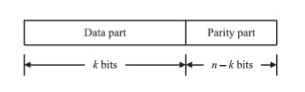
\includegraphics[width=0.55\linewidth]{figures/systematic_form.png}}
\caption{Κωδική λέξη σε συστηματική μορφή}
\label{fig:systematic form}
\end{figure}

Στη συστηματική μορφή, η κωδική λέξη χωρίζεται στο τμήμα μηνύματος (\en{data part}) και στο πλεονάζον τμήμα ελέγχου (\en{parity part}). Το τμήμα μηνύματος αποτελείται από τα $k$ αναλλοίωτα ψηφία πληροφορίας και το πλεονάζον τμήμα ελέγχου, από τα $n-k$ \en{bits} ελέγχου ισοτιμίας. Ολόκληρος ο γραμμικός μπλοκ κώδικας $(n,k)$ βρίσκεται σε \textit{συστηματική} μορφή, όταν μπορέι να οριστεί πλήρως από έναν $k \times n$ γεννήτορα πίνακα με την παρακάτω μορφή:

\begin{equation}
\mathbf{G} = \left[\mathbf{P}\;\;\mathbf{I}_{k}\right]= 
\left[\underbrace{\begin{matrix}
p_{0,0} & p_{0,1} & \cdots & p_{0,n-k-1} \\
p_{1,0} & p_{1,1} & \cdots & p_{1,n-k-1} \\
\vdots & \vdots & \ddots & \vdots \\
p_{k-1,0} & p_{k-1,1} & \cdots & p_{k-1,n-k-1}
\end{matrix}}_{\text{\en{\textbf{P}} πίνακας}}\;
\underbrace{\begin{matrix}
1 & 0 & \cdots & 0 \\
0 & 1 & \cdots & 0 \\
\vdots & \vdots & \ddots & \vdots \\
0 & 0 & \cdots & 1
\end{matrix}}_{\text{$k\times k$ $\mathbf{I}_k$ μοναδιαίος πίνακας}}\right]
\label{eq:generator matrix systematic form}
\end{equation}

Όπως διαπιστώνεται και από την εξίσωση \ref{eq:generator matrix systematic form}, ο γεννήτορας πίνακας $\mathbf{G}$, που για απλότητα μπορεί να γραφτεί ως $\mathbf{G}=\left[\mathbf{P}\;\;\mathbf{I}_k\right]$, αποτελείται από δύο υποπίνακες, έναν $k\times (n-k)$ υποπίνακα $\mathbf{P}$ στα αριστερά και έναν $k\times k$ μοναδιαίο πίνακα $\mathbf{G}_k$ στα δεξιά \cite{ryan2009channel}.

Η συστηματική μορφή του πίνακα $\mathbf{G}$ έχει σημαντικά πλεονεκτήματα καθώς σε κάθε κωδική λέξη, τα \en{bits} πληροφορίας παραμένουν αναλλοίωτα στις αρχικές $k$ θέσεις της. Μειώνεται συνεπώς η πολυπλοκότητα κωδικοποίησης, αφού χρειάζεται να υπολογιστούν μόνο τα σύμβολα του πλεονάζοντος τμήματος ελέγχου.

Αντίστοιχα, όταν ο γεννήτορας πίνακας είναι σε συστηματική μορφή, ο πίνακας ελέγχου ισοτιμίας διαμορφώνεται ως εξής:

\begin{equation}
\mathbf{H}=\left[\mathbf{I}_{n-k}\;\;\mathbf{P^T}\right]
=\begin{bmatrix}
1 & 0 & \cdots & 0 & \; & p_{0,0} & p_{1,0} & \cdots & p_{k-1,0} \\
0 & 1 & \cdots & 0 & \; & p_{0,1} & p_{1,1} & \cdots & p_{k-1,1} \\
\vdots & \vdots & \ddots & \vdots  & \; & \vdots & \vdots & \ddots & \vdots \\
0 & 0 & \cdots & 1 & \; & p_{0,n-k} & p_{1,n-k} & \cdots & p_{k-1,n-k}
\end{bmatrix}
\end{equation}

Θεωρείται όπως και παραπάνω το μήνυμα πληροφορίας $\mathbf{u} = (u_0, u_1, ..., u_{k-1})$. Αν εφαρμοστεί η εξίσωση \ref{eq:check equation}, όταν ο πίνακας $\mathbf{G}$ είναι σε συστηματική μορφή, τα στοιχεία της κωδικές λέξης $\mathbf{v}$ προκύπτουν:

\begin{equation}
\begin{aligned}
v_{n-k+i}=u_i\;\;\ & \forall\;\;0\leq i < k  \\
v_j=u_0p_{0,j}+u_1p_{1,j}+\cdots+u_{k-1}p_{k-1,j}\;\; & \forall\;\;0\leq j < n-k
\end{aligned}
\label{eq:systematic codeword formation}
\end{equation}

Οι εξισώσεις \ref{eq:systematic codeword formation} δείχνουν πως τα πρώτα $k$ \en{bits} της κωδικής λέξης παραμένουν ίδια και τα υπόλοιπα $n-k$ αποτελούν γραμμικό συνδυασμό των \en{bits} πληροφορίας. Επίσης οι ίδιες εξισώσεις μπορούν να προκύψουν και από τον πίνακα $\mathbf{H}$ (σε συστηματική μορφή), εφαρμόζοντας στοιχειώδεις γραμμικούς μετασχηματισμούς. Αποδεικνύεται συνεπώς το πολύ χρήσιμο συμπέρασμα που αναφέρθηκε ήδη πως δηλαδή, ένας γραμμικός μπλοκ κώδικας ορίζεται πλήρως από τον \en{parity-check} πίνακα και γι\textquotesingleαυτό καλείται \en{parity-check} κώδικας.

Επίσης φανερώνονται τα πλεονεκτήματα που προσφέρει η συστηματική μορφή. Λιγότερων υπολογισμών, καθώς το μήνυμα πληροφορίας παραμένει ατόφιο και μειωμένης πολυπλοκότητας αφού υπολογίζεται εύκολα ο πίνακας ελέγχου ισοτιμίας $\mathbf{H}=\left[\mathbf{I}_{n-k}\;\;\mathbf{P^T}\right]$ και από αυτόν κάθε κωδική λέξη.



\section{Πολυπλοκότητα}
Σε αυτό το σημείο ίσως υπάρξει κομμάτι για την πολυπλοκότητα.
% \en{\lipsum[1]}

% From the generator and parity-check representation of a linear code we see that its
% description complexity is atmost min˜rn2, (1−r)n2 bits, where r is the rate of the
% code. Further, from (1.20) it is clear that the encoding task, i.e., the mapping of the
% information block onto the codeword, can be accomplished in O(n2) operations.

% ¿e notion
% of complexity on the other hand is fuzzy. As we have just discussed, we can easily
% distinguish polynomial and exponential complexity
